%% This is file 'chapter2.tex'
%% It is included by hhuthesis-example.tex for hhuthesis.
%%
%% Copyright(C) 2020-2021, Wenhan Cao
%% College of Water Conservancy and Hydropower Engineering, Hohai University.
%%
%% Version:v2.0.0
%% Last update: April 7th, 2021.
%%
%% Home Page of the Project: https://github.com/caowenhan/thesis
%%
%% This file may be distributed and / or modified under the conditions of the
%% LaTeX Project Public License, either version 1.3c of this license or (at your
%% option) any later version. The latest version of this license is in:
%%
%% http://www.latex-project.org/lppl.txt
%%
%% and version 1.3c or later is part of all distributions of LaTeX version
%% 2008/05/04 or later.
%%
\chapter{实验配置}
\label{chap:inverseproblem}
\section{MeGaT实验方案}
MeGaT(MeV Gamma-ray Telescope)探测系统作为新一代高气压时间投影室(TPC)技术的创新性应用,其特殊的架构旨在突破MeV伽马天文长期面临的空间分辨与灵敏度瓶颈。该系统采用双模态复合探测器设计,
通过高气压TPC+Micromegas电子径迹成像模块与像素化半导体/闪烁体量能器的协同工作,从而实现对康普顿散射过程的全事件重建:
\subsection{TPC+Micromegas电子径迹重建模块}
	TPC+Micromegas电子径迹重建模块是MeGaT探测系统的核心部件,其主要功能是实现低能量分辨率、大视场、低角度分辨率的MeV伽马射线探测。该模块采用高气压TPC技术,结合Micromegas电子径迹成像技术,
	实现对MeV伽马射线的低能量分辨率探测。该模块的设计和制造工艺对MeGaT探测系统的性能有重要影响,是MeGaT探测系统的关键技术之一。\par
\subsection{像素化半导体/闪烁体量能器}
	像素化半导体/闪烁体量能器是MeGaT探测系统的辅助部件,其主要功能是实现对MeV伽马射线的高能量分辨率探测。该模块采用像素化半导体/闪烁体量能器技术,结合TPC+Micromegas电子径迹重建模块,
	实现了对MeV伽马射线的高能量分辨率探测。该模块的设计和制造工艺对MeGaT探测系统的性能有重要影响,是MeGaT探测系统的关键技术之一。
	基于像素化半导体/闪烁体量能器技术,实现对MeV伽马射线的高能量分辨率探测,能量分辨率达到1\%(FWHM),探测效率达到10\%。
	\begin{figure}
		\centering
		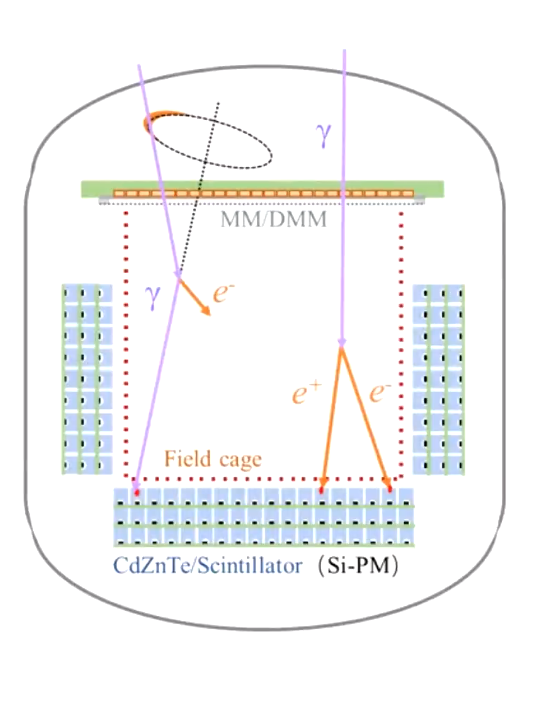
\includegraphics[width=0.55\textwidth]{figures/MeGaT.png}
		\caption{MeGaT探测系统概念图}
	\end{figure}

\section{MeGaT 实验原理}
MeGaT(MeV伽马射线望远镜)项目的核心原理基于康普顿散射成像技术,通过高气压时间投影室(TPC)与像素化碲锌镉(CZT)探测器的协同工作,实现对MeV能段伽马射线的高精度探测与重建。
其工作原理可分为以下几个关键步骤:首先,入射伽马光子在TPC内与氙气原子发生康普顿散射,产生高能电子和散射光子;TPC模块利用10 bar高气压环境延长电子径迹,
并通过Micromegas探测器对电子的三维径迹进行高分辨率重建(空间分辨率0.3 mm),精确确定散射顶点坐标(误差±0.5 mm)和电子出射方向(角度误差<1°)。
随后,散射光子进入CZT探测器,通过光电效应或多次康普顿作用沉积能量,CZT凭借其高原子序数(Z=48)和像素化设计(像素间距0.5 mm),在1-10 MeV能段实现优于1\%的
能量分辨率和亚毫米级位置精度。通过TPC记录的散射角($\theta$)与CZT测量的剩余光子能量($E_{\gamma'}$),结合康普顿公式$E_{\gamma} = \frac{E_{\theta}}{1-\cos (\theta)}$,
MeGaT系统可精确反推入射伽马光子的初始能量($E_{\gamma}$)和方向($\theta$)。此外,TPC与CZT的时间符合测量(时间窗<10 ns)可有效剔除宇宙线等非关联事件,将本底噪声抑制至10⁴量级,
显著提升信噪比。MeGaT还采用贝叶斯反演算法(BIO-COM)优化康普顿锥重建,将开角不确定性从传统方法的±20°压缩至±4°,进一步提高了角度分辨率

\section{MeGaT 实验方案性能模拟优化}


描述明渠一维非恒定流的基本方程为一维Saint-Venant 方程组:
\begin{equation}
	\frac{\partial Q}{\partial x}+B_{W}\frac{\partial Z}{\partial t}=q
\end{equation}
\begin{equation}
	\frac{\partial Q}{\partial t}+2u\frac{\partial Q}{\partial x}+(gA-Bu^{2})\frac{\partial Z}{\partial x}-u^{2}\frac{\partial A}{\partial x}+g\frac{n^{2} |u|Q}{R^{4/3}}=0
\end{equation}
\noindent 式中,$t$为时间坐标;$x$为空间坐标;……\par
……\par
……

\section{ TPC 探测器构建与性能研究}


\section{数据与模拟对比分析}
\subsection{电子学噪声测试}
由于读出芯片在制造工艺上的固有缺陷,读出电荷的噪声是不可避免的。在实际测量中,噪声会对信号的测量精度产生影响,因此需要对读出电荷的噪声进行测试。\par


\subsection{探测器X-RAY准直测试}


\subsection{探测器X-RAY能谱测试}


\subsection{}



\section{讨论与总结}
为了验证上述计算方法的可靠性,通常借用正问题的解来构造反问题。即先进行正问题计算,用其结果验证反问题的解。\par
……\par
……\par
计算结果见表\ref{tab:parameter}。

\begin{table}[H]\small	%\small用于控制表格内字体大小为5号字
	\centering
	\caption{参数理论值与最优解} \label{tab:parameter}
	\begin{tabular*}{0.75\textwidth}{@{\extracolsep{\fill}}cccc}
		\toprule
		\multicolumn{1}{l}{} & b1     & b2     & b3     \\\midrule
		理论解                  & 22     & 18     & 16     \\
		最优解1                 & 21.986 & 18.048 & 15.997 \\
		最优解2                 & 21.997 & 18.011 & 15.999 \\ \bottomrule
	\end{tabular*}%
\end{table}


……\par
……
\section{本章小结}
本章采用平原河网三级联合解法水量模型模拟河网的水力要素,建立了平原河网
水量模型,对位于长江下游的南通河网进行了模拟运算。\par
……\par
……
